\documentclass[11pt]{article}
\usepackage[margin=1in]{geometry}
\usepackage[T1]{fontenc}
\usepackage{lmodern,microtype}
\usepackage{amsmath,amssymb,graphicx,booktabs,array,siunitx,xcolor}
\usepackage{tikz}
\usetikzlibrary{arrows.meta,positioning,fit,calc}
\usepackage{caption,subcaption,float,placeins}
\usepackage[numbers,sort&compress]{natbib}
\usepackage[hidelinks]{hyperref}
\definecolor{navy}{RGB}{35,68,105}
\graphicspath{{figures/}}
\sisetup{detect-all,group-separator={,},output-decimal-marker={.}}
\title{\textbf{EcoHydroGraph: Hydro--ecological temporal graph learning for sparse river water-quality reconstruction}}
\author{Zhaochen Yang\\[2pt]\small Draft manuscript --- September 2026}
\date{}
\begin{document}
\maketitle

\begin{abstract}
River monitoring networks rarely observe every water-quality indicator at every station and month. These gaps are structured by river connectivity, watershed ecology, hydrologic conditions, and sampling schedules. We introduce \textbf{EcoHydroGraph}, a temporal river-graph model that combines a spatial graph encoder, watershed ecological features, hydroclimatic inputs, and a causal gated recurrent unit. We evaluate separate models for dissolved organic carbon (DOC), pH, and specific conductance on an audited 357-station, 654-month river-network cohort under random, temporal, and spatial missingness. In a five-seed matched comparison, EcoHydroGraph reduces DOC mean absolute error by 37.5--47.2\% and specific-conductance error by 38.8--57.2\% relative to the matched snapshot graph model. pH gains are smaller (0.5--3.8\%) and depend on the missingness regime. Window diagnostics show that most pH and conductance gains appear by six months, whereas DOC changes little with window length. The results show that analyte-specific hydro--ecological temporal context can improve sparse water-quality reconstruction.
\end{abstract}
\paragraph{Keywords:} river monitoring; water-quality reconstruction; graph neural network; ecological informatics; temporal memory; dissolved organic carbon

\section{Introduction}
Long-term river monitoring networks provide broad spatial and temporal coverage, but observations remain sparse and irregular. Stations differ in sampling frequency, programs change over time, and access or instrumentation creates gaps. These gaps are embedded in a river network, a watershed ecological context, and a changing hydrologic regime. This limits the use of raw records for carbon-cycle analysis, salinity assessment, acid--base characterization, extreme-event detection, and comparisons among watersheds.

Conventional interpolation uses local spatial or temporal similarity. Tabular machine-learning models add environmental covariates while treating station-month records as independent samples. Graph neural networks encode relational structure \citep{kipf2017,hamilton2017}, yet many water-quality applications remain snapshot models. Recurrent models capture temporal persistence \citep{cho2014}, but commonly process stations as independent sequences and omit the river network. The open problem is to combine spatial graph structure, ecological context, and hydroclimatic temporal memory while testing the result under the distinct ways a monitoring network becomes incomplete.

We develop EcoHydroGraph. A spatial river-graph encoder combines station inputs, edge attributes, and ecological features at each month. A causal GRU integrates the current representation with the preceding eleven months. Here causal describes the information-flow constraint that a prediction at month $t$ receives no future-month labels; it is not a causal-inference claim. Separate models are trained for DOC, pH, and specific conductance.

Our contributions are threefold: (i) a hydro--ecological temporal graph model for sparse station-month reconstruction; (ii) evidence that temporal information has analyte- and missingness-dependent value, with large gains for DOC and specific conductance and smaller gains for pH; and (iii) a matched evaluation framework that separates random, temporal, and spatial missingness and measures the useful history length. The design isolates the value of temporal context by keeping the spatial encoder and target masks fixed between the snapshot and temporal models.

\section{Materials and Methods}
\subsection{Cohort, targets, and inputs}
The audited ST357 cohort contains 357 stream stations, 324 river-network edges, and 654 monthly time points. DOC and specific conductance use a log1p target transform; pH is standardized on the raw scale using training cells only. Monthly inputs contain temperature, discharge, visibility flags, seasonal sine/cosine terms, static station coordinates, ecological regime features, and target-value/visibility channels. The graph input contains the frozen river edge set and edge attributes.

\subsection{Missingness and visibility}
We evaluate four scenarios: \textit{random gaps}, which hide individual observed cells; \textit{unobserved-period extrapolation}, which hides all target observations after the temporal cutoff; \textit{observation-assisted extrapolation}, which retains a subset of post-cutoff observations as context; and \textit{unmonitored stations}, which withholds target observations at selected stations. Role cells are intersected with each analyte's observed-label mask. Training and context labels can populate the input under the role definition. Validation labels remain hidden during fitting and early stopping; test labels are used only for final evaluation. Snapshot and temporal models use identical target masks and query cells.

\subsection{EcoHydroGraph}
The spatial trunk is a two-layer transport graph encoder with hidden width 64, ecological encoding, and dropout 0.1. It is applied to every monthly station graph. The resulting node representations enter a one-layer GRU with hidden width 64 and a 12-month causal window. The final recurrent representation is mapped through the prediction head to the target analyte. The snapshot baseline uses the same spatial trunk without the temporal wrapper. Figure~\ref{fig:architecture} summarizes the architecture.

\begin{figure}[t]\centering
\resizebox{\linewidth}{!}{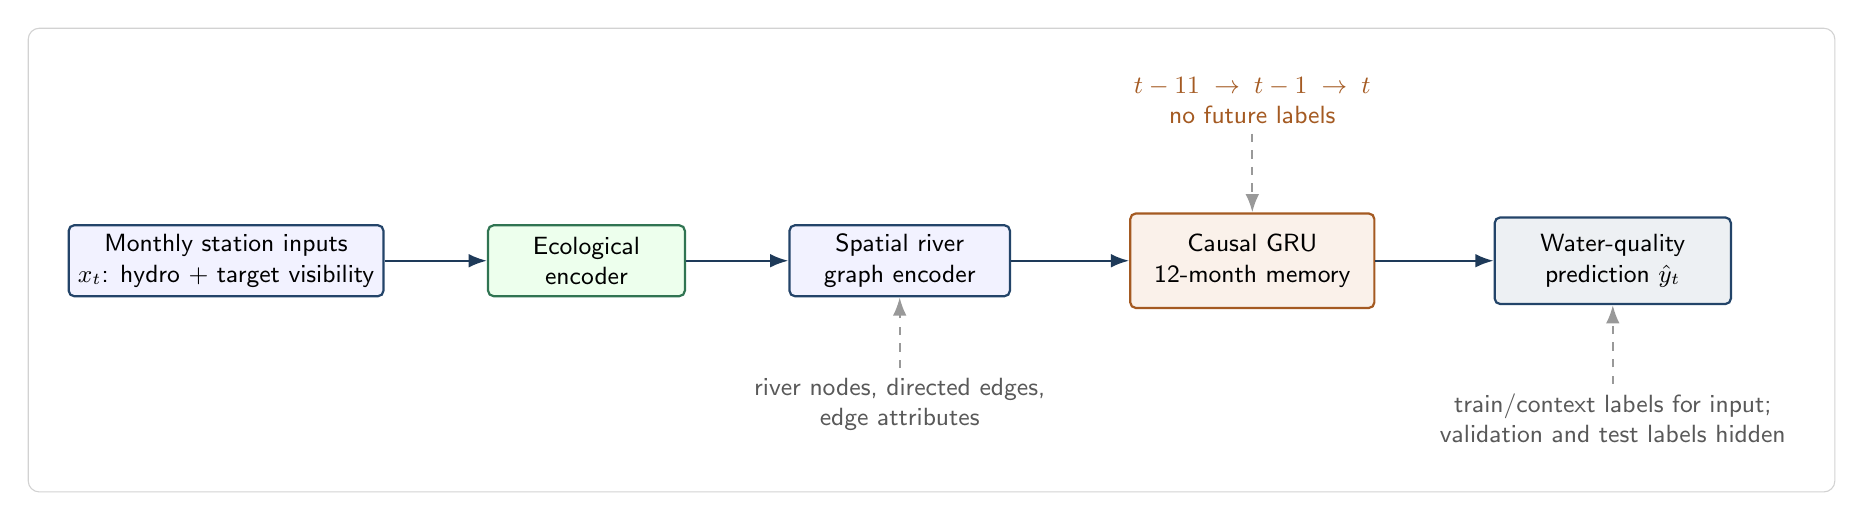
\begin{tikzpicture}[
  font=\sffamily\small,
  >=Latex,
  box/.style={draw=navy, rounded corners=2pt, thick, align=center, minimum height=9mm, minimum width=28mm, fill=blue!5},
  eco/.style={draw=forest, rounded corners=2pt, thick, align=center, minimum height=9mm, minimum width=25mm, fill=green!7},
  time/.style={draw=orange!80!black, rounded corners=2pt, thick, align=center, minimum height=12mm, minimum width=31mm, fill=orange!10},
  output/.style={draw=navy, rounded corners=2pt, thick, align=center, minimum height=11mm, minimum width=30mm, fill=navy!8},
  arrow/.style={->, thick, draw=navy!85!black},
  dashedarrow/.style={->, thick, dashed, draw=gray!80}
]
\definecolor{navy}{RGB}{35,68,105}
\definecolor{forest}{RGB}{48,116,82}
\definecolor{orange}{RGB}{205,112,42}

\node[box] (x0) {Monthly station inputs\\$x_t$: hydro + target visibility};
\node[eco, right=13mm of x0] (eco) {Ecological\\encoder};
\node[box, right=13mm of eco] (g0) {Spatial river\\graph encoder};
\node[time, right=15mm of g0] (gru) {Causal GRU\\12-month memory};
\node[output, right=15mm of gru] (pred) {Water-quality\\prediction $\hat y_t$};

\draw[arrow] (x0) -- (eco);
\draw[arrow] (eco) -- (g0);
\draw[arrow] (g0) -- (gru);
\draw[arrow] (gru) -- (pred);

\node[below=9mm of g0, align=center, text=gray!70!black] (graphnote) {river nodes, directed edges,\\edge attributes};
\draw[dashedarrow] (graphnote.north) -- (g0.south);

\node[above=10mm of gru, align=center, text=orange!80!black] (memory) {$t-11 \;\rightarrow\; t-1 \;\rightarrow\; t$\\no future labels};
\draw[dashedarrow] (memory.south) -- (gru.north);

\node[below=10mm of pred, align=center, text=gray!70!black] (roles) {train/context labels for input;\\validation and test labels hidden};
\draw[dashedarrow] (roles.north) -- (pred.south);

\node[fit=(x0)(eco)(g0)(gru)(pred)(graphnote)(memory)(roles), inner sep=5mm, draw=gray!35, rounded corners=4pt] {};
\end{tikzpicture}

}
\caption{\textbf{EcoHydroGraph architecture.} Monthly hydroclimatic, ecological, and target-visibility inputs are encoded on the river graph. The spatial encoder is applied to the preceding eleven months and the current month, after which a causal GRU produces the current prediction.}
\label{fig:architecture}
\end{figure}

\subsection{Training and evaluation}
Primary comparisons use five seeds (42--46) and the matched 10-epoch, patience-3 budget for both models. The primary metric is MAE on hidden query cells; RMSE, $R^2$, log-space error, and train-derived Q90 tail MAE are secondary. Tails with fewer than 20 query cells are flagged unstable. Errors are averaged across seeds at each query cell before 2,000 paired station- or month-clustered bootstrap replicates. The primary uncertainty table reports station-clustered 95\% intervals for the paired MAE difference; month-clustered intervals are retained in the analysis files. Relative reduction is $100(1-\mathrm{MAE}_{\mathrm{EcoHydroGraph}}/\mathrm{MAE}_{\mathrm{snapshot}})$.

\section{Results}
\subsection{EcoHydroGraph improves sparse reconstruction}
Table~\ref{tab:main} gives the five-seed matched comparison. EcoHydroGraph improves DOC in all four regimes, with reductions from 37.5\% in unmonitored stations to 47.2\% in observation-assisted extrapolation. Specific conductance shows reductions from 38.8\% in unmonitored stations to 57.2\% in observation-assisted extrapolation. Both analytes improve for all five seeds in every regime. The largest gains occur in the two temporal extrapolation scenarios, where the query month is separated from observed target history.

The paired station-clustered intervals in Table~\ref{tab:ci} remain below zero for every DOC and conductance scenario. For pH, the intervals are below zero in random gaps and both temporal extrapolation scenarios, but include zero for unmonitored stations. This pattern is consistent with an analyte- and missingness-dependent temporal benefit rather than a uniform improvement.

pH shows a smaller effect: reductions range from 0.5\% in unmonitored stations to 3.8\% in observation-assisted extrapolation. Random gaps and both temporal extrapolation scenarios improve for four of five seeds. Reconstruction at unmonitored stations is close to parity, with the station-clustered interval including zero.

\begin{table*}[t]\centering\caption{Five-seed matched comparison. Positive reduction favors EcoHydroGraph.}\label{tab:main}\scriptsize
\setlength{\tabcolsep}{3pt}
\begin{tabular}{lp{2.8cm}rrrr}\toprule
Analyte & Scenario & \shortstack{Snapshot\\MAE} & \shortstack{EcoHydroGraph\\MAE} & \shortstack{Reduction\\(\%)} & \shortstack{Better\\seeds}\\\midrule
DOC&Random gaps&4.285&2.625&38.75&5/5\\
DOC&Strict temporal&2.679&1.417&47.12&5/5\\
DOC&Context-assisted temporal&2.679&1.413&47.24&5/5\\
DOC&Unmonitored stations&6.198&3.876&37.47&5/5\\\midrule
pH&Random gaps&0.347&0.335&3.53&4/5\\
pH&Strict temporal&0.313&0.302&3.58&4/5\\
pH&Context-assisted temporal&0.312&0.300&3.77&4/5\\
pH&Unmonitored stations&0.286&0.284&0.51&3/5\\\midrule
Specific conductance&Random gaps&683.2&374.8&45.14&5/5\\
Specific conductance&Strict temporal&572.7&247.9&56.71&5/5\\
Specific conductance&Context-assisted temporal&568.9&243.5&57.19&5/5\\
Specific conductance&Unmonitored stations&996.4&609.4&38.84&5/5\\\bottomrule
\end{tabular}\end{table*}

\begin{table}[t]\centering
\caption{Station-clustered 95\% bootstrap intervals for the paired MAE difference (EcoHydroGraph minus snapshot). Negative values favor EcoHydroGraph.}
\label{tab:ci}\scriptsize
\setlength{\tabcolsep}{3pt}
\begin{tabular}{llrr}\toprule
Analyte & Scenario & $\Delta$ MAE & 95\% CI\\\midrule
DOC&Random gaps&$-1.660$&$[-1.894,-1.415]$\\
DOC&Strict temporal&$-1.263$&$[-1.722,-0.763]$\\
DOC&Context-assisted temporal&$-1.266$&$[-1.725,-0.740]$\\
DOC&Unmonitored stations&$-2.322$&$[-2.770,-1.900]$\\\midrule
pH&Random gaps&$-0.012$&$[-0.019,-0.007]$\\
pH&Strict temporal&$-0.011$&$[-0.017,-0.005]$\\
pH&Context-assisted temporal&$-0.012$&$[-0.018,-0.006]$\\
pH&Unmonitored stations&$-0.001$&$[-0.005,0.002]$\\\midrule
Specific conductance&Random gaps&$-308.4$&$[-345.1,-272.8]$\\
Specific conductance&Strict temporal&$-324.8$&$[-396.2,-247.1]$\\
Specific conductance&Context-assisted temporal&$-325.4$&$[-396.9,-245.3]$\\
Specific conductance&Unmonitored stations&$-387.0$&$[-443.2,-321.8]$\\\bottomrule
\end{tabular}\end{table}

\begin{figure}[t]\centering
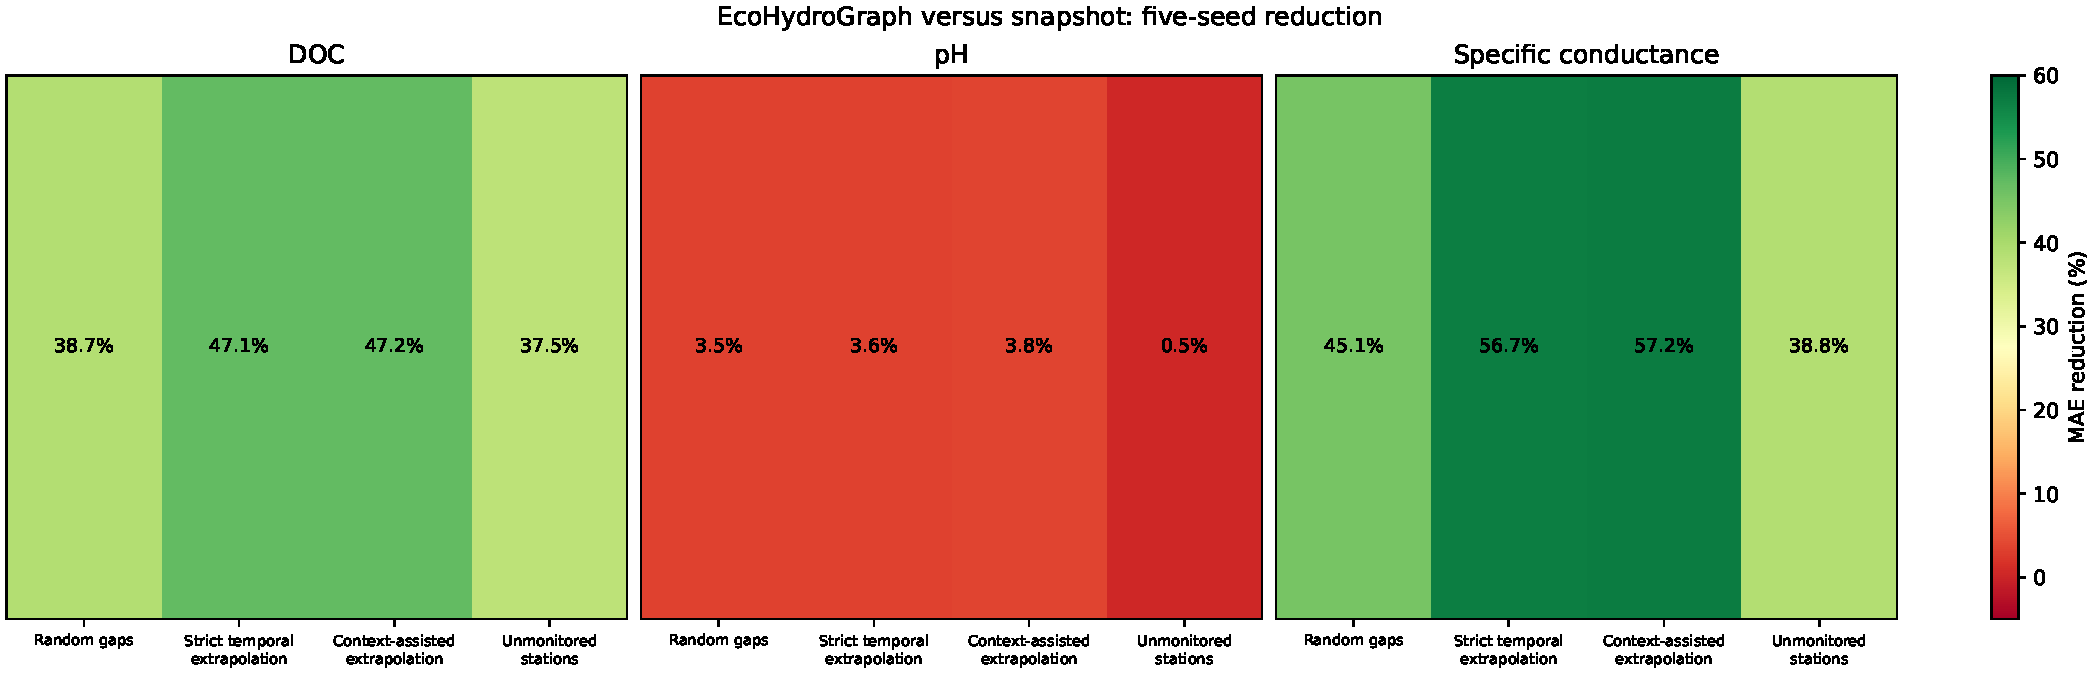
\includegraphics[width=\linewidth]{reconstruction_improvement.pdf}
\caption{\textbf{Analyte- and regime-specific improvement.} Relative MAE reduction of EcoHydroGraph relative to the matched snapshot graph model.}
\label{fig:heatmap}\end{figure}

\subsection{Temporal history length has analyte-specific value}
The window diagnostic compares 1, 3, 6, and 12 months in the two temporal extrapolation scenarios using three matched seeds. Mean MAE decreases from 1.420 to 1.415 for DOC, from 0.362 to 0.301 for pH, and from 279.12 to 245.75 for specific conductance. Most pH and conductance improvement appears by six months, while DOC is nearly flat. We retain 12 months as the common working configuration.

\begin{table}[t]\centering\caption{Mean MAE across the two temporal extrapolation scenarios by temporal lookback.}\label{tab:window}\small
\begin{tabular}{lrrrr}\toprule
Analyte&1 month&3 months&6 months&12 months\\\midrule
DOC&1.420&1.419&1.417&1.415\\
pH&0.362&0.319&0.305&0.301\\
Specific conductance&279.12&255.19&247.72&245.75\\\bottomrule
\end{tabular}\end{table}

\begin{figure}[t]\centering
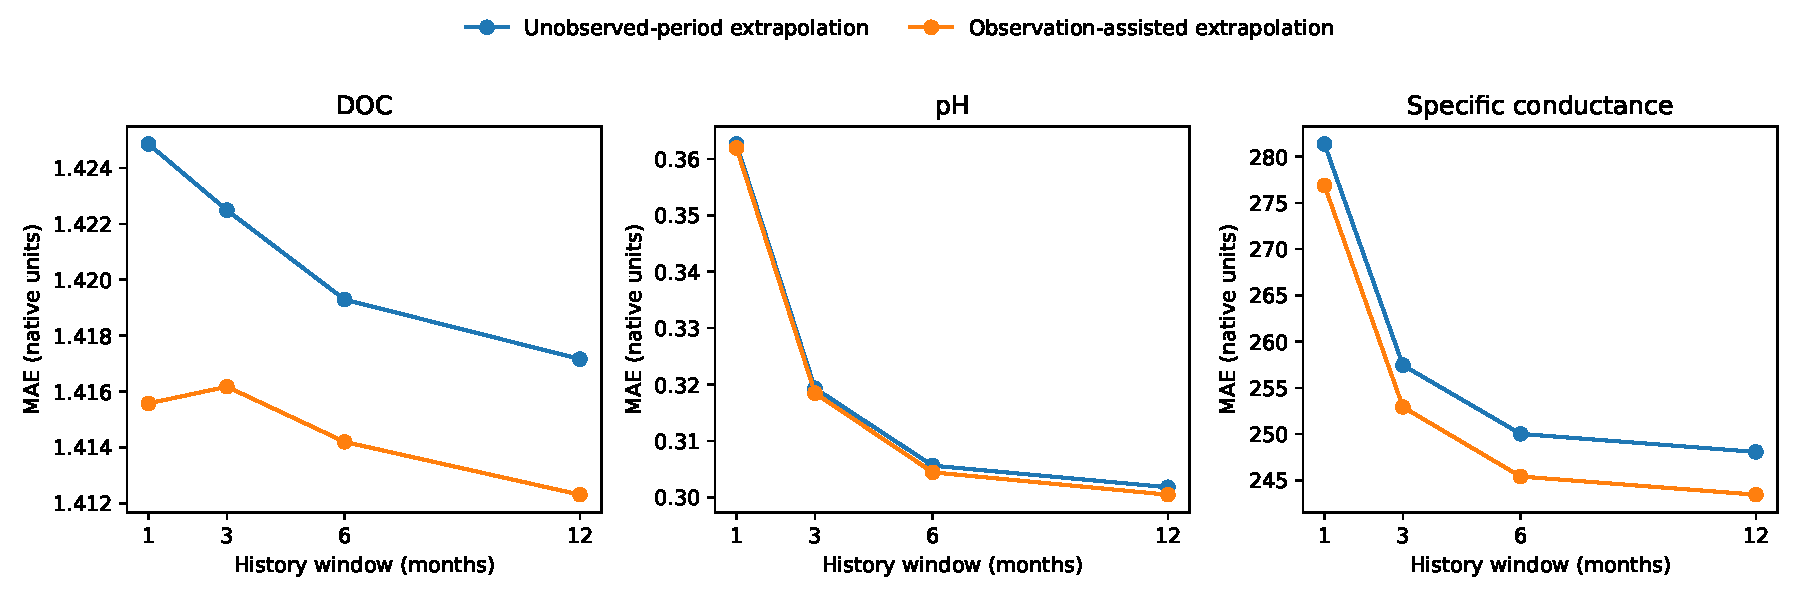
\includegraphics[width=\linewidth]{history_window.pdf}
\caption{\textbf{Temporal window diagnostic.} Longer history improves pH and specific conductance, with diminishing gains beyond six months. DOC changes little.}
\label{fig:window}\end{figure}

\subsection{Longer history matters more than one isolated channel}
The reverse-history and hydro-only arms remain within 0.6\% of the full temporal model in the three-seed diagnostic. The current-only control is 20.9\% worse for pH and 13.8\% worse for specific conductance in the two temporal extrapolation scenarios, while DOC changes by 0.5\%. These results identify the amount of temporal context as useful for pH and conductance. They do not isolate strict chronological order from the amount of history, and they do not establish that target-analyte history is the source of the gain.

\begin{figure}[t]\centering
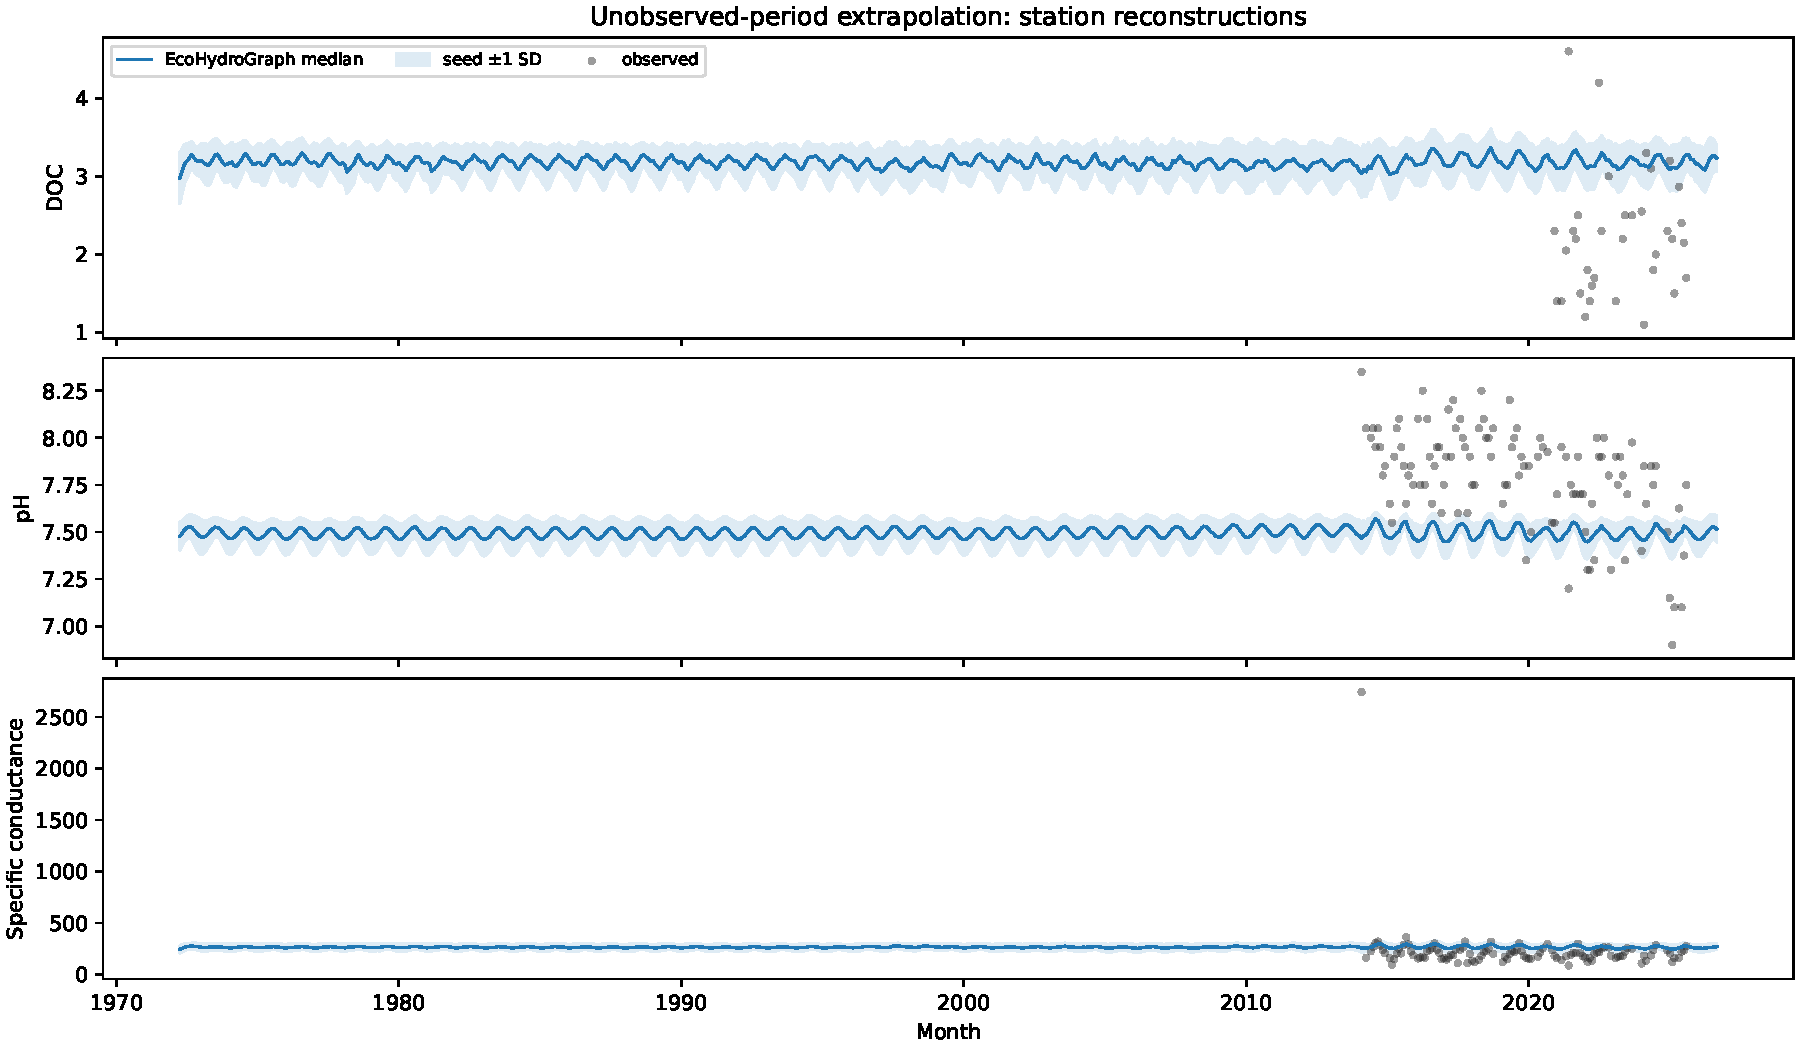
\includegraphics[width=\linewidth]{unobserved_period_traces.pdf}
\caption{\textbf{Descriptive station traces under unobserved-period extrapolation.} Five-seed EcoHydroGraph median predictions, observed values, and seed dispersion for one fixed data-availability-selected station per analyte.}
\label{fig:trace}\end{figure}

\subsection{Spatially heterogeneous reconstruction error}
The five-seed ensemble produces a full station-month reconstruction for every analyte and regime. Figure~\ref{fig:map} shows test-cell error under unobserved-period extrapolation by station. Error is spatially heterogeneous, and the scale differs among analytes.

\begin{figure}[t]\centering
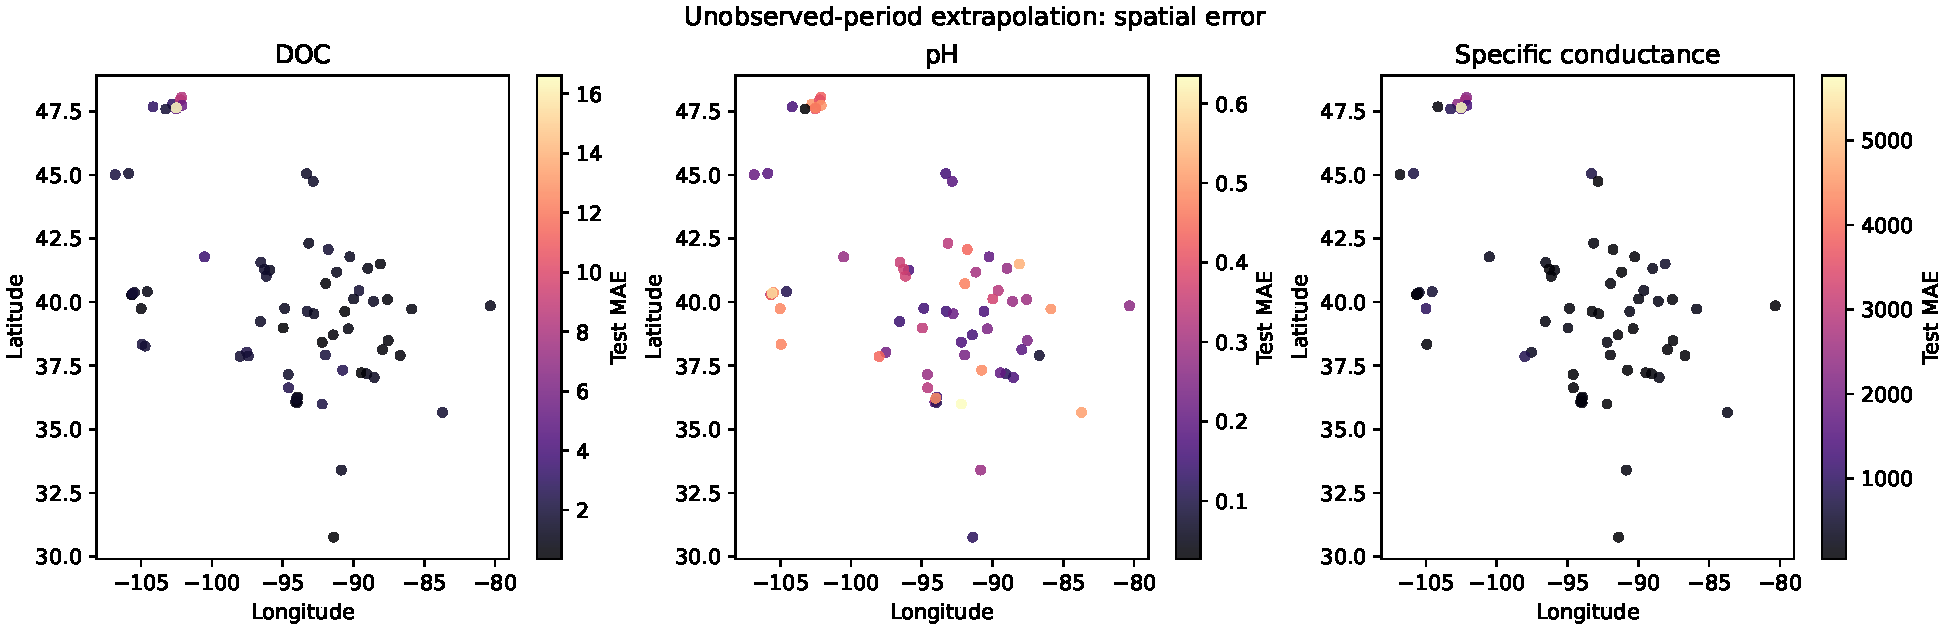
\includegraphics[width=\linewidth]{unobserved_period_spatial_error.pdf}
\caption{\textbf{Spatial error under unobserved-period extrapolation.} Station-level MAE for the five-seed EcoHydroGraph median reconstruction.}
\label{fig:map}\end{figure}

\FloatBarrier
\section{Discussion}
The central finding is that hydro--ecological temporal memory improves sparse water-quality reconstruction, with value determined by the target analyte and missingness process. DOC and specific conductance show large and consistent gains, especially under temporal extrapolation. pH shows smaller gains and near-parity under spatial station holdout. The same model therefore reveals heterogeneity in the recoverable information of water-quality variables.

The graph provides the spatial context in which ecological and hydroclimatic inputs are interpreted. The headline result is the performance pattern created by jointly modeling river structure, ecology, and time. The window curve suggests that a six-month implementation may offer most of the benefit for pH and conductance, while the 12-month configuration remains the best common model. Because the spatial trunk is held fixed, this comparison isolates the temporal extension rather than ranking all possible spatial models.

The reconstruction products expose where the model is less informative. pH gains are modest, and tail metrics are unstable in scenarios with very few high-value query cells. Ensemble seed spread is a model-dispersion diagnostic rather than a calibrated prediction interval. External-basin replication and a channel-factorial experiment are natural next tests.

\section{Conclusion}
EcoHydroGraph combines river-network structure, watershed ecology, and hydro-temporal memory for sparse water-quality reconstruction. On ST357, it substantially improves DOC and specific-conductance reconstruction across random, temporal, and spatial missingness, while pH benefits more modestly. The recoverable memory of a river monitoring system is analyte-specific, providing a basis for model-assisted gap filling between direct observations.

\section*{Data and code availability}
Analysis products, provenance records, and scripts are maintained in the project repository. Main tables are in \path{experiments/phase4_transfer/temporal_h2x_v1/t8_synthesis/}; five-seed products and figures are in \path{experiments/phase4_transfer/temporal_h2x_v1/t9_products/}.

\section*{Acknowledgements}Draft placeholder.

\bibliographystyle{plainnat}
\begin{thebibliography}{9}\small
\bibitem[Kipf and Welling(2017)]{kipf2017} Kipf, T. N. and Welling, M. (2017). Semi-supervised classification with graph convolutional networks. \emph{ICLR}.
\bibitem[Hamilton et~al.(2017)Hamilton, Ying, and Leskovec]{hamilton2017} Hamilton, W. L., Ying, R., and Leskovec, J. (2017). Inductive representation learning on large graphs. \emph{NeurIPS}, 30.
\bibitem[Cho et~al.(2014)Cho et~al.]{cho2014} Cho, K. et~al. (2014). Learning phrase representations using RNN encoder--decoder for statistical machine translation. \emph{EMNLP}, 1724--1734.
\bibitem[Reichstein et~al.(2019)Reichstein et~al.]{reichstein2019} Reichstein, M. et~al. (2019). Deep learning and process understanding for data-driven Earth system science. \emph{Nature}, 566, 195--204.
\end{thebibliography}
\end{document}
